\documentclass[11pt,a4paper]{article}
\usepackage[T1]{fontenc}
\usepackage[utf8]{inputenc}
\usepackage[margin=1in]{geometry}
\usepackage{amsmath,amssymb,amsthm}
\usepackage{mathpartir}
\usepackage{stmaryrd}
\usepackage{booktabs}
\usepackage{tabularx}
\usepackage{array}
\usepackage{longtable}
\usepackage{enumitem}
\usepackage{listings}
\usepackage{xcolor}
\usepackage[expansion=false]{microtype}
\usepackage{tikz}
\usetikzlibrary{arrows.meta,positioning,fit,calc}
\usepackage[htt]{hyphenat}
\usepackage[hidelinks,pdftitle={F1R3COMB: a compiler from kernel rho to the name-free rho combinators}]{hyperref}
\setlength{\emergencystretch}{3em}

\newcommand{\code}[1]{\texttt{#1}}
\newcommand{\Comb}{\textsc{F1R3Comb}}
\newcommand{\Kind}{\textsc{K1ndl1ng}}
\newcommand{\Camp}{\textsc{CampF1R3}}
\newcommand{\Bell}{\textsc{B3ll0ws}}
\newcommand{\Fx}{\textsc{F1R3x}}
\newcommand{\Rhobots}{\textsc{Rhobots}}
\newcommand{\MUST}{\textsc{must}}
\newcommand{\MUSTNOT}{\textsc{must not}}
\newcommand{\SHOULD}{\textsc{should}}
\newcommand{\SHOULDNOT}{\textsc{should not}}
\newcommand{\MAY}{\textsc{may}}

\newcommand{\quo}[1]{@#1}
\newcommand{\drp}[1]{{*}#1}
\newcommand{\inp}[3]{\mathsf{for}(\,#1 \leftarrow #2\,)#3}
\newcommand{\out}[2]{#1!(#2)}
\newcommand{\nil}{\mathbf{0}}
\newcommand{\enc}[1]{\llbracket #1 \rrbracket}
\newcommand{\nequiv}{\equiv_{\mathcal{N}}}
\newcommand{\bisim}{\approx}
\newcommand{\nms}[1]{\mathcal{N}^{*}(#1)}
\newcommand{\Nsort}{\mathsf{N}}
\newcommand{\Psort}{\mathsf{P}}

\newcommand{\mm}{\mathsf{m}}
\newcommand{\dd}{\mathsf{d}}
\newcommand{\kk}{\mathsf{k}}
\newcommand{\fw}{\mathsf{fw}}
\newcommand{\bl}{\mathsf{b}_{\mathsf{l}}}
\newcommand{\br}{\mathsf{b}_{\mathsf{r}}}
\newcommand{\sy}{\mathsf{s}}
\newcommand{\ev}{\mathsf{e}}
\newcommand{\qq}{\mathsf{q}}
\newcommand{\cons}{\mathsf{cons}}
\newcommand{\Lft}{\mathsf{L}}
\newcommand{\Rgt}{\mathsf{R}}
\newcommand{\red}{\longrightarrow}
\newcommand{\wred}{\longrightarrow^{*}}
\newcommand{\scong}{\equiv}
\newcommand{\Atm}{\mathcal{A}}
\newcommand{\shapes}{\mathrm{shapes}}
\newcommand{\Cl}{\mathrm{Cl}}
\newcommand{\ALLOC}{\mathrm{ALLOC}}
\newcommand{\ERECT}{\mathrm{ERECT}}
\newcommand{\inst}{\mathsf{inst}}

\theoremstyle{definition}
\newtheorem{definition}{Definition}[section]
\newtheorem{requirement}[definition]{Requirement}
\newtheorem{decision}[definition]{Decision}
\newtheorem{obligation}[definition]{Obligation}
\newtheorem{hazard}[definition]{Hazard}
\newtheorem{erratum}[definition]{Erratum}
\newtheorem{remark}[definition]{Remark}
\newtheorem{example}[definition]{Example}
\theoremstyle{plain}
\newtheorem{proposition}[definition]{Proposition}
\newtheorem{lemma}[definition]{Lemma}

\lstset{
  basicstyle=\ttfamily\footnotesize,
  columns=fullflexible,
  keepspaces=true,
  breaklines=true,
  frame=leftline,
  framesep=6pt,
  xleftmargin=8pt,
  rulecolor=\color{black!30},
  showstringspaces=false,
}

\title{\textbf{\Comb}\\[1mm]
\large A compiler from kernel rho to the name-free rho combinators,\\
and a machine that runs the result\\[2mm]
\normalsize Specification v0.5}
\author{F1R3FLY.io}
\date{23 September 2026}

\begin{document}
\maketitle

\begin{abstract}
\noindent
\cite{draft3} has been revised again, and this revision does something the
previous ones did not: it takes a finding of v0.4 and pushes it much further
than v0.4 did, with the result that v0.4's proposed construction is refuted by
name.

v0.4 observed that $\ERECT$ as \cite[Def.~6.8]{draft3} states it violates the
single-address-input discipline, and proposed a two-stage erection ---
single-input chains at static channels, erecting a per-instance erector at
address-derived channels, which erects the unit. \cite[\S6.6]{draft3} shows
that this regresses without a base case: the erector is itself an atom
mentioning several leaves, so erecting \emph{it} faces the same choice.
\cite[Prop.~6.17]{draft3} makes the obstruction structural --- under the
discipline every reachable atom holds at most one occurrence of an address, so
\emph{no} construction from the fixed-arity family erects an atom mentioning
two leaves --- and \cite[Lem.~6.19]{draft3} concludes that a rule of
multiplicity at least two is required. Requirement~5.16 of v0.4 is withdrawn
in Remark~\ref{rem:twostagegone}.

\cite[\S6.7]{draft3} gives two rules that supply the multiplicity: curried
path-indexed constructors, and the context-instantiation atom $\inst$, and
recommends $\inst$ on measurements. This specification takes the choice as a
seam with the curried scheme as default (Decision~\ref{dec:scheme}), for three
reasons the measurements do not cover: the experiment's arms are the broken
scheme and $\inst$, with no curried arm, so the data shows ``not literal''
rather than ``$\inst$ over curried''; $\inst$ reintroduces substitution
under quotation as a machine primitive, which is the operation the
constructor family exists to simulate and the reason the machine could be
\Camp{} with a three-line matcher; and \cite{logic}'s revision~2 restates
$\Atm_{\mathrm{full}}$ in the curried style, so $\inst$ leaves the logic's
grammar and the lattice report without a home. Section~\ref{sec:schemes} also
corrects one row of \cite[\S6.7]{draft3}'s comparison table: the curried
scheme does \emph{not} still need the allocation tree, because path
derivation is internal to its rule, which narrows the engineering gap
considerably.

Key words \MUST, \MUSTNOT, \SHOULD, \MAY{} are used in the sense of RFC~2119.
\end{abstract}

\tableofcontents

%======================================================================
\section{Purpose and scope}\label{sec:purpose}

\subsection{The gap}

\cite{draft3} defines a translation from the rho calculus into the repaired
combinators, in two phases, and proves it correct as full abstraction relative
to encoded contexts. \cite{logic} gives the spatial-behavioural logic over the
same calculus. Neither has been run. The properties a paper translation may
leave up to bisimilarity --- which address, which static channel, which
representative of a constructed name, which presentation --- are properties an
implementation may not leave open, because they decide whether two
independently compiled terms can speak to one another.

The \code{campf1r3} workspace is a complete executive for kernel rho:
\code{k1ndl1ng-parse} and \code{k1ndl1ng-norm} take text to a canonical normal
form, \code{campf1r3-core} is the store, \code{b3ll0ws} interprets the normal
form, and \code{f1r3x} drives them. It knows nothing of combinators. \Comb{}
is the missing arrow, plus the smallest machine that can run its output.

\subsection{What exists today}

\begin{center}
\begin{tabularx}{\linewidth}{@{}l>{\raggedright\arraybackslash}X@{}}
\toprule
Artefact & What it gives this project\\
\midrule
\code{rho-combinators-draft3} & The target as an operational theory
(\S3.2--3.3), the two presentations and the argument between them (\S3.3,
\S4), the constructor family (Def.~3.8), erection at a computed name
(Rem.~3.11), the positional-naming bug (\S6.1), phase one (\S6.2), phase two
(\S6.3), the permutation discipline (\S6.4, Def.~6.10, Lem.~6.11), phase-two
freshness (\S6.5, Lem.~6.14), the multiplicity obstruction (\S6.6,
Prop.~6.17, Lem.~6.19), the two erection schemes (\S6.7, Rem.~6.22), the
correctness lemmas (\S7), the lattice (\S9)\\
\code{phase2.py}, \code{phase2-results.txt} & The measurements behind
\cite[Rem.~6.22]{draft3}: literal erection mixes in 29--50 runs out of 50; the
context scheme mixes in none; $D_{x}$ at seven parallel steps and sixteen new
names per unfolding over two hundred unfoldings\\
\code{rhocomb-logic} (draft~2 rev.~2) & The logic; the presentation decision
(Dec.~2.3), what B costs it (Prop.~2.4, Rem.~2.5), drop elimination
(Lem.~2.8), $\nequiv$ decided (Prop.~2.10), the weighted atom count
(Def.~6.6), occupancy in linear time, and revision~2's restatement of
$\Atm_{\mathrm{full}}$ as a program's shape set\\
\code{k1ndl1ng-spec} & K0 = pure rho; the AST, the normal form, its encoding
and hashing (Def.~2.6, Req.~2.7, Prop.~6.9)\\
\code{campf1r3-spec} & The store: $D$, $W$, $I$, produce/consume/install,
joins, profiles, replay\\
\code{bytecode-or-normal-form} & Why code must never be a channel key unless
the compiler is canonical\\
\code{campf1r3} (the repository) & The eight crates, no external
dependencies\\
\bottomrule
\end{tabularx}
\end{center}

\subsection{Nomenclature}\label{sec:nomen}

\begin{center}
\begin{tabularx}{\linewidth}{@{}l>{\raggedright\arraybackslash}X@{}}
\toprule
Term & Meaning here\\
\midrule
\emph{source} & K0 of \cite{k1ndl1ng}, the rho calculus of
\cite[\S2]{draft3} modulo Obligation~\ref{obl:srcagree}\\
\emph{target}, $\mathrm{RC}$ & The theory of \cite[\S3]{draft3}: two sorts,
nine atom shapes plus the constructor family, $\nil$, par, quote, drop, no
binders\\
$\mathrm{RC}^{\nu}$ & The target extended with
$(\mathsf{new}\,z)P$; the codomain of phase one and the compiler's
intermediate representation\\
\emph{presentation A}, \emph{B} & \cite[\S3.3]{draft3}; A adds
$\drp{\quo{p}} = p$ and sorts message payloads as names\\
\emph{router} & $\dd,\kk,\fw,\bl,\br,\sy$\\
\emph{constructor} & $\cons_{A}$ for an atom shape $A$, per
\cite[Def.~3.8]{draft3}\\
\emph{address} & The name an instance receives at run time and allocates
beneath\\
\emph{leaf}, $\sigma\!\cdot\!w$ & An allocated name, at path $w$ beneath
address $\sigma$\\
\emph{static channel} & A name appearing in the phase-two image itself,
shared by every instance\\
\emph{unit} & One quotation's worth of phase-one output: the top-level term,
or the body of one input, phase-two-compiled on its own\\
\emph{instance} & One run-time copy of a unit, at one address\\
\emph{link} & The atom emitted for one occurrence, per Table~\ref{tab:links}\\
\bottomrule
\end{tabularx}
\end{center}

\subsection{Goals and non-goals}

\begin{enumerate}[leftmargin=1.6em]
\item A total, canonical, terminating compiler implementing
\cite[Def.~6.3 and~6.8]{draft3}, with every degree of freedom in them closed.
\item A target representation with a canonical encoding and content hash, so
that $\nequiv$ is a 32-byte comparison, and an intermediate representation
carrying the phase-one binder.
\item A machine that runs target terms by instantiating \Camp{}.
\item Differential testing against \Bell, including the two-instance
interleaving that \cite[\S6.1]{draft3} and \cite[Rem.~6.10]{draft3} make the
crux of correctness.
\item A term type and an occupancy report \cite{logic} can build on.
\item No external dependencies, \code{forbid(unsafe\_code)}, WebAssembly-clean.
\end{enumerate}

\noindent
Out of scope: the logic itself; K1 and K2; the $\pi$ route; decompilation;
cost accounting; the matrix encoding of the reduction graph; optimisation
beyond \cite[Rem.~6.4]{draft3}.

%======================================================================
\section{Which presentation}\label{sec:which}

\cite[\S3.3]{draft3} gives two sound presentations and \cite[Rem.~3.2]{draft3}
shows they cannot be mixed piecemeal. A compiler cannot hold both: the term
type, the datum type, the tag table and the decision procedure for $\nequiv$
all differ.

\begin{center}
\begin{tabularx}{\linewidth}{@{}l>{\raggedright\arraybackslash}X>{\raggedright\arraybackslash}X@{}}
\toprule
& Presentation A & Presentation B\\
\midrule
$\mm$ payload sort & $\Nsort$ & $\Psort$\\
$\mathsf{eval}$ & $\ev(a) \mid \mm(a,v) \red \drp{v}$ &
  $\ev(a) \mid \mm(a,p) \red p$\\
$\drp{-}$ in a term & eliminable; absent from normal forms
  (\cite[Lem.~2.8]{logic}) & irreducible; needed\\
$\quo{-}$ injective & yes, on normal forms (\cite[Prop.~2.10]{logic}) & no
  (\cite[Prop.~2.4(ii)]{logic})\\
$\nequiv$ decided by & byte equality of the encoding & a separate
  normalisation, strictly coarser\\
$\cons_{\qq}$ & $\quo{\qq(v_{1},\drp{v_{2}})}$: available, but its
  correctness is the equation & $\qq(\quo{p_{1}},p_{2})$: direct, the sorts
  already fit (\cite[Rem.~3.9]{draft3})\\
Logic support & full & needs a receptivity primitive
  (\cite[Rem.~2.5]{logic})\\
\bottomrule
\end{tabularx}
\end{center}

\begin{decision}[\Comb{} implements presentation A]\label{dec:presA}
Unchanged from v0.2, and now overdetermined. The reasons of v0.2 stand: the
logic is a logic for A and under B cannot distinguish a store from a message;
$\quo{-}$ is injective only under A and \Camp{} keys channels by the encoding;
\cite[Def.~3.3]{draft3} writes the translation in A's notation; the
representation is smaller; and \code{k1ndl1ng-norm} already implements A on
the source side.
\end{decision}

\begin{remark}[v0.3's fourth reason is withdrawn]\label{rem:withdrawn}
v0.3 argued that phase two must erect the gate's storage atom and that only A
can build the constructor for it, making phase two A-only.
\cite[Def.~3.8]{draft3} and \cite[Rem.~3.9]{draft3} settle it the other way.
The member exists in both: under B it is
$\cons_{\qq}(a,b,c) \mid \mm(a,p_{1}) \mid \mm(b,p_{2}) \red
\mm(c,\qq(\quo{p_{1}},p_{2}))$, where the sorts already fit; under A it must
be written $\quo{\qq(v_{1},\drp{v_{2}})}$, coercing a name back to a process,
which denotes the intended atom only because $\drp{\quo{p}} = p$. So this is a
third place the presentations come apart, and it leans mildly towards B. It
does not move the decision: within A the coercion is sound by the equation A
asserts, so the cost is presentational rather than real, and the three reasons
above are untouched. It is recorded because v0.3 claimed the opposite, and a
reader of both documents is entitled to know which is right.
\end{remark}

\begin{remark}[The \S4 argument of \protect\cite{draft3}, still outstanding]
\label{rem:s4}
v0.2 \S2.3 answered \cite[\S4]{draft3}'s reading of the F1R3FLY normaliser as
evidence for B: sorting a parallel composition is the monoid laws, common to
both; de Bruijn indexing applies to source binders and the combinators have
none; and the one presentation-specific rewrite the code performs,
$\drp{\quo{P}} \to P$, is A's equation. That section is unchanged in the
revision, so the point stands as written.
\end{remark}

\begin{requirement}[Presentation is a compile-time parameter]\label{req:pseam}
\code{presentation-b} \MUST{} be a cargo feature, off by default, coupling the
equation, the payload sort and the $\mathsf{eval}$ rule in one switch
(\cite[Rem.~3.2]{draft3}). It \MUST{} be recorded in every artefact header and
a deploy \MUST{} diagnose a mismatch. Both presentations admit the whole
translation, including the erection of storage atoms
(Remark~\ref{rem:withdrawn}), so the seam has no structural exclusion and
\MUST{} be exercised across the whole corpus (Obligation~\ref{obl:AB}).
\end{requirement}

%======================================================================
\section{The source language}\label{sec:source}

\begin{center}
\begin{tabular}{@{}lll@{}}
\toprule
\cite[Def.~2.1]{draft3} & K0 & \code{k1ndl1ng-norm} \code{Node}\\
\midrule
$\nil$ & \code{Nil} & \code{Nil}\\
$P \mid Q$ & \code{P | Q} & \code{Par(Vec<Norm>)}, sorted, no \code{Nil}\\
$\out{x}{P}$ & \code{x!(P)} & \code{Send\{chan, persistent:false, args:[P]\}}\\
$\inp{y}{x}{P}$ & \code{for(y <- x)\{P\}} & \code{Receive\{binds:[b], body\}}\\
$\drp{x}$ & \code{*x} & \code{Eval(Name)}\\
$\quo{P}$ & \code{@P} & \code{Name::Quote(Norm)}\\
\bottomrule
\end{tabular}
\end{center}

\begin{requirement}[Source level and closedness]\label{req:level}
\Comb{} \MUST{} accept exactly K0, invoking \code{k1ndl1ng\_parse} with
\code{Level::K0}, and \MUST{} reject every K1 and K2 form with a distinct
diagnostic. The term \MUST{} be closed: no \code{FreeVar}, no
\code{FreeName}. \code{Name::Unforgeable} \MUST{} be rejected, because the
target has no name former for it; grounding \MUST{} be by quotation.
\end{requirement}

\begin{obligation}[The source presentations agree on guarded-drop terms]
\label{obl:srcagree}
\cite[\S2]{draft3} states the source congruence without $\drp{\quo{P}} \scong
P$; \cite[Def.~2.6]{k1ndl1ng} asserts it and \code{Norm::eval} applies it
eagerly. For $P$ guarded-drop (\cite[Def.~2.5]{draft3}) no subterm
$\drp{\quo{Q}}$ occurs in $P$ or any reduct (\cite[Lem.~2.6]{draft3}), so the
rewrite never fires and the congruences coincide. This \MUST{} be proved; it
is what licenses compiling a \Kind{} normal form against \cite[\S2]{draft3}.
\end{obligation}

\begin{requirement}[Guarded-drop check]\label{req:guarded}
The compiler \MUST{} verify the guarded-drop property on the \emph{tree},
before normalisation, since \code{Norm::eval} has already collapsed
$\drp{\quo{Q}}$ by the time the normal form exists. Under
Decision~\ref{dec:presA} violations are warnings and compilation \MAY{}
proceed; under \code{presentation-b} they \MUST{} be errors.
\end{requirement}

\begin{decision}[Compile the normal form, not the tree]
The compiler's input is \code{k1ndl1ng\_norm::Norm}, with the sole exception of
Requirement~\ref{req:guarded}. Compiling the tree would make the output depend
on how the author happened to write a parallel composition, and
Obligation~\ref{thm:canon} would be false.
\end{decision}

%======================================================================
\section{The target calculus}\label{sec:target}

\subsection{Formation, equations, rules}

From \cite[\S3.2]{draft3}, with $a,b,c,f : \Nsort$ and $p,q : \Psort$:

\[
\begin{array}{l@{\qquad}l@{\qquad}l}
 \mm(a,v) & \bl(a,b) & \cons_{A}(a_{1},\dots,a_{n},f)\\
 \dd(a,b,c) & \br(a,b) & \cons_{\mid}(a,b,c)\\
 \kk(a) & \sy(a,b,c) & \\
 \fw(a,b) & \ev(a) & \\
 \qq(a,p) & \nil \,,\ \ p \mid q & \quo{p} : \Nsort \,,\ \ \drp{a} : \Psort
\end{array}
\]

\begin{requirement}[The drop and the guard are distinct constructors]
\label{req:noconflation}
$\drp{-}$ and $\ev$ \MUST{} be distinct constructors of the target type and no
code path \MAY{} convert one into the other. \cite[Prop.~3.5]{draft3} needs
the conflation as a hypothesis; with them separate, an arbitrary running
process cannot match a guard however many equations the theory carries. A
representation sharing one tag between them \MUSTNOT{} be used even with a
discriminating flag.
\end{requirement}

\begin{definition}[Equations, \cite{draft3} Def.~3.1]\label{def:teqns}
$(\Psort,\mid,\nil)$ is an abelian monoid; $\quo{\drp{a}} = a$; and, under A,
$\drp{\quo{p}} = p$.
\end{definition}

\begin{requirement}[Drop elimination]\label{req:dropelim}
Orient the equations left to right. By \cite[Lem.~2.8]{logic} the system is
terminating and confluent and a closed normal form contains no $\drp{-}$. The
smart constructors \MUST{} apply both rewrites at construction, so that every
\code{Term} in existence is in normal form and every traversal may assume a
flat multiset of atoms. Under \code{presentation-b},
Requirement~\ref{req:nodropB} inverts this.
\end{requirement}

\begin{definition}[Rules, \cite{draft3} Def.~3.3 and~3.8]\label{def:tred}
\[
\begin{array}{l}
 \mathsf{dist} : \dd(a,b,c) \mid \mm(a,v) \red \mm(b,v) \mid \mm(c,v)\\
 \mathsf{kill} : \kk(a) \mid \mm(a,v) \red \nil\\
 \mathsf{forward} : \fw(a,b) \mid \mm(a,v) \red \mm(b,v)\\
 \mathsf{bind}_{\mathsf{l}} : \bl(a,b) \mid \mm(a,v) \red \fw(v,b)\\
 \mathsf{bind}_{\mathsf{r}} : \br(a,b) \mid \mm(a,v) \red \fw(b,v)\\
 \mathsf{synch} : \sy(a,b,c) \mid \mm(a,v) \red \fw(b,c)\\
 \mathsf{eval} : \ev(a) \mid \mm(a,v) \red \drp{v}\\
 \mathsf{quote} : \fw(a,b) \mid \qq(a,p) \red \mm(b,\quo{p})\\
 \mathsf{make}_{\mid} : \cons_{\mid}(a,b,c) \mid \mm(a,\quo{p}) \mid
   \mm(b,\quo{r}) \red \mm(c,\quo{(p \mid r)})\\
 \mathsf{make}_{A} : \cons_{A}(a_{1},\dots,a_{n},f) \mid \mm(a_{1},v_{1})
   \mid \cdots \mid \mm(a_{n},v_{n}) \red \mm(f,\quo{A(\vec v)})
\end{array}
\]
closed under parallel composition and the equations, subjects matched up to
$\nequiv$.
\end{definition}

\begin{requirement}[The rule table is generated, not written]\label{req:rules}
With $\mathsf{make}_{A}$ a schema over atom shapes, the rule table \MUST{} be
\emph{derived} from the shape table: one row per shape, giving arity and
argument sorts, from which both the atom and its constructor are generated.
Hand-writing thirteen-plus rows invites exactly the divergence
\cite[Rem.~3.4]{draft3} records. The machine's step function \MUST{} be a
dispatch over the generated table.
\end{requirement}

\begin{requirement}[The three departures]\label{req:departures}
\cite[Rem.~3.4]{draft3}'s corrections \MUST{} each carry a test. The binders
produce forwarders: $\bl(a,b) \mid \mm(a,v) \red \fw(v,b)$ and
$\br(a,b) \mid \mm(a,v) \red \fw(b,v)$. A version producing a message
duplicates $\mathsf{forward}$, collapses a lattice edge, and breaks
occurrence kinds (o1) and (o2). $\fw$ is binary. A constructor's delivery
channel is in its own argument list and distinct from its inputs.
\end{requirement}

\subsection{The constructor family}\label{sec:family}

\cite[Def.~3.8]{draft3} replaces the four constructors of the previous
revision with one per atom shape, and \cite[Rem.~3.13]{draft3} makes the
enlargement compulsory rather than fastidious: phase two erects allocated
atoms by Remark~3.11, which calls for a constructor at every shape the
compiled output contains.

\begin{requirement}[The family is computed, and is one level deep]
\label{req:family}
The family \MUST{} be computed, per program, as
\[
  \mathcal{F}(P) \;=\; \{\,\cons_{A} \;:\; A \in \shapes(\enc{P}),\ \text{some
  atom of shape } A \text{ in } \enc{P}\ \text{mentions a bound name}\,\}
\]
where $\enc{P}$ is the phase-one image. It \MUSTNOT{} be taken as the
transitive closure of the signature under $\cons$. \cite[Rem.~6.15]{draft3}
now states why the recursion terminates at one level per program: $\ERECT$
erects only phase-one atoms, so the shapes needed are those of atoms
mentioning a bound name, and the $\cons_{A}$ atoms doing the erecting appear
in the phase-two image, which is never itself erected. The compiler
\MUST{} emit $\mathcal{F}(P)$ in the artefact header, since
Requirement~\ref{req:shortcuts} and the lattice report both consume it.
\end{requirement}

\begin{requirement}[$\cons_{\qq}$ and the shapes with a process argument]
\label{req:consq}
\cite[Def.~3.8]{draft3} now states the member for a shape with a process
argument, $\cons_{\qq}(a,b,c) \mid \mm(a,p_{1}) \mid \mm(b,p_{2}) \red
\mm(c,\qq(\quo{p_{1}},p_{2}))$, in presentation~B's sorting, with
\cite[Rem.~3.9]{draft3} giving A's reading
$\quo{\qq(v_{1},\drp{v_{2}})}$. The implementation \MUST{} provide it in the
sorting of the selected presentation, generated from the shape table like
every other member (Requirement~\ref{req:rules}), and under A \MUST{} apply
drop elimination to the result so that the erected atom is in normal form
(Requirement~\ref{req:dropelim}). The two readings \MUST{} produce the same
erected atom on the corpus, which is a cheap check on the coercion and is the
executable form of \cite[Rem.~3.9]{draft3}.
\end{requirement}

\begin{requirement}[Erecting a storage atom whose payload is allocated]
\label{req:qpayload}
\cite[Ex.~6.9]{draft3} erects $\qq(b,\ev(c))$, in which the payload itself
mentions an allocated name. The compiler \MUST{} therefore build the payload
first --- $\cons_{\ev}$ at $c$'s chain, yielding $\quo{\ev(c)}$ --- and feed
that name to $\cons_{\qq}$, which means $\cons_{\ev}$ is in $\mathcal{F}(P)$
for every unit containing an input, independently of
Requirement~\ref{req:shortcuts}. The family computation \MUST{} include the
shapes reached through gate payloads and not only the shapes of top-level
atoms.
\end{requirement}

\subsection{Representation, encoding, hashing}

\begin{requirement}[Encoding]\label{req:enc}
A target term \MUST{} have a canonical byte encoding built bottom-up in the
smart constructors and cached on the node, in the style of
\cite[\S6]{k1ndl1ng}: tag byte, then LEB128 lengths and counts, then children.
Parallel components \MUST{} be ordered by bytewise comparison of their own
encodings, with $\nil$ absent. The content hash \MUST{} be BLAKE2b-256 of the
encoding.
\end{requirement}

\begin{requirement}[Tags: a shape table, not a flat enumeration]\label{req:tags}
Target tags \MUST{} occupy a block disjoint from the source tags of
\cite[\S6]{k1ndl1ng}. Because the constructor family is a schema, the tag
space \MUST{} be structured as a shape byte plus a one-bit constructor
flag, so that $\cons_{A}$'s tag is derived from $A$'s and a new shape costs no
tag negotiation. The reserved layout:
\end{requirement}

\begin{center}
\begin{tabular}{@{}ll@{}}
\toprule
Tag & Shape\\
\midrule
\code{0x30} & $\nil$\\
\code{0x31} & par, $n \geq 2$ components\\
\code{0x32}--\code{0x3B} & the atoms: $\mm,\dd,\kk,\fw,\bl,\br,\sy,\ev,\qq$,
  reserved\\
\code{0x40} & $\quo{p}$, name former\\
\code{0x41} & $\drp{a}$, \code{presentation-b} only; rejected by the decoder
  under A\\
\code{0x50}--\code{0x5B} & $\cons_{A}$, where $A$ is the shape at
  \code{0x30}+$(t-\code{0x50})$; $\cons_{\mid}$ is \code{0x51}\\
\bottomrule
\end{tabular}
\end{center}

\begin{requirement}[Name equivalence is a hash comparison]\label{req:neq}
Under A, $a \nequiv b$ iff their encodings are equal iff their content hashes
are equal modulo collision (\cite[Prop.~2.10]{logic}). The machine \MUST{}
match subjects by content hash and \MUSTNOT{} implement a separate $\nequiv$
procedure. This discharges corrigendum~5 of \cite[\S11]{draft3}.
\end{requirement}

\begin{requirement}[No variables in the target]\label{req:novars}
The \emph{target} node type \MUSTNOT{} have a bound-variable, free-variable or
wildcard case, nor a $\mathsf{new}$ case. The binder lives in the
intermediate representation of Section~\ref{sec:ir} and nowhere else; a
phase-two image that still carries one is a compiler bug, and the type system
\MUST{} make it unrepresentable.
\end{requirement}

\begin{requirement}[Under B, the opposite on drops]\label{req:nodropB}
With \code{presentation-b}, $\drp{\quo{p}} \to p$ \MUSTNOT{} be applied, the
drop node \MUST{} be retained, every traversal \MUST{} carry a descent case
for it (\cite[Prop.~2.4(iii)]{logic}), and the term type \MUSTNOT{} be routed
through \code{k1ndl1ng\_norm::Norm::eval}.
\end{requirement}

%======================================================================
\section{The two-phase translation}\label{sec:twophase}

\subsection{The bug, and why the specification had it too}
\label{sec:thebug}

\cite[\S6.1]{draft3} exhibits
\[
  W \;=\; \inp{z}{b}{(\drp{z} \mid \drp{z})} \mid \out{b}{R}
      \mid \out{a}{X} \mid \out{a}{Y},
  \qquad R = \inp{y}{a}{\out{y}{\drp{y}}},
\]
on which a translation whose apparatus names are functions of syntactic
position is unsound: $\ev$ instantiates the same compiled text at both drop
sites, so both instances of $R$ carry the same proxy $c$, and after the links
fire nothing pairs a forwarder with the message from its own copy. A run
yields $\enc{\out{\quo{X}}{Y}} \mid \enc{\out{\quo{Y}}{X}}$, which an encoded
observer distinguishes from the source.

\begin{remark}[v0.2 was a positional scheme]\label{rem:v2bug}
This specification is among the affected artefacts, and it is worth being
exact about how. v0.2's Decision~4.6 made the seed a function of the source
name, $\enc{\quo{P}} := \quo{\enc{P}_{\quo{P}}}$, and Requirement~4.7
allocated seed powers by canonical path within a unit. Both were aimed at
\emph{canonicity} --- the same source must compile to the same bytes --- and
they achieved it. Canonicity is precisely what makes the bug bite: if the same
source always yields the same apparatus names, then two run-time instances of
one compiled occurrence necessarily share them. The invariant v0.2 secured and
the invariant correctness needs were in direct opposition, and v0.2 did not
notice. The two-phase translation resolves the opposition by moving apparatus
names out of the compiled artefact entirely: the artefact is closed, and
freshness happens at run time (Section~\ref{sec:canon}).
\end{remark}

\begin{requirement}[$W$ is the first regression test]\label{req:Wtest}
$W$ \MUST{} be a golden test in \code{f1r3comb-check} before any other
translation test, run under both \Bell{} and the machine, asserting the
observation at $\enc{\quo{X}}$. It is the term the translation exists to get
right, and any future change to naming \MUST{} be measured against it.
\end{requirement}

\subsection{Phase one}\label{sec:ir}

\begin{definition}[\cite{draft3} Def.~6.3]\label{def:phase1}
On names, $\enc{\quo{P}} := \quo{\enc{P}}$. On processes,
\[
\begin{array}{rcl}
  \enc{\nil} &=& \nil\\
  \enc{P \mid Q} &=& \enc{P} \mid \enc{Q}\\
  \enc{\out{x}{P}} &=& \mm(\enc{x}, \quo{\enc{P}})\\
  \enc{\inp{y}{x}{P}} &=& (\mathsf{new}\,p_{0},\dots,p_{k},c_{1},\dots,c_{k})\,
    \big(D(\enc{x};\vec p) \mid G(p_{0}, B) \mid L_{1} \mid \cdots \mid L_{k}\big)
\end{array}
\]
with $G(p,S) := (\mathsf{new}\,b,c)(\sy(p,b,c) \mid \qq(b,S) \mid \ev(c))$,
$D$ the duplicator chain under $(\mathsf{new}\,q_{1},\dots,q_{k-1})$,
$o_{1},\dots,o_{k}$ the free occurrences of $y$ in $P$, and $L_{i}$ and the
residue in $B$ given by Table~\ref{tab:links}.
\end{definition}

\begin{requirement}[Phase one is a homomorphism, and that is the point]
\label{req:phase1hom}
Phase one \MUST{} be implemented as a structural homomorphism on the source
normal form, with no name allocation of any kind: bound names are binder
occurrences in the intermediate representation, not names. It is therefore
canonical without argument (Obligation~\ref{thm:canon}), and the entire
freshness question is deferred to phase two, where it belongs.
\end{requirement}

\begin{requirement}[The intermediate representation]\label{req:irtype}
$\mathrm{RC}^{\nu}$ \MUST{} have its own Rust type in its own crate, with a
$\mathsf{new}$ node and de Bruijn indices for its bound names --- not a
\code{Term} with an extra variant, because
Requirement~\ref{req:novars} must remain enforceable by the type system. The
IR \MUST{} support scope extrusion and $\alpha$-equivalence, and \MAY{} be
encoded and hashed for testing, but \MUSTNOT{} be deployable.
\end{requirement}

\begin{requirement}[Occurrence enumeration order]\label{req:occorder}
\cite[Def.~6.3]{draft3} says only ``let $o_{1},\dots,o_{k}$ enumerate the free
occurrences''. The order decides which bound name is $c_{1}$, hence which leaf
it is allocated in phase two, hence the bytes of the output. Occurrences
\MUST{} be enumerated by ascending byte offset in the encoding of the
receive's body, which is a function of the source normal form and therefore
canonical.
\end{requirement}

\begin{requirement}[A unit is a quotation]\label{req:units}
Scope extrusion cannot move a $\mathsf{new}$ out of a quotation, and the body
$B$ of an input travels as the payload of $\qq(b,B)$. Phase two is therefore
applied \emph{per quotation}: the top-level term is one unit, and the body of
each input is another, compiled on its own. \cite[Def.~6.8]{draft3}'s ``bound
names $z_{1},\dots,z_{n}$ under a single $\mathsf{new}$'' is to be read as the
binders of one unit after extrusion within that unit.
\end{requirement}

\subsection{Phase two}\label{sec:phase2}

\begin{definition}[Allocation, \cite{draft3} Def.~6.6]\label{def:alloc}
Fix $K := \quo{\mm(\quo{\nil},\quo{\nil})}$,
$\Lft\sigma := \quo{\mm(\sigma,\quo{\nil})}$ and
$\Rgt\sigma := \quo{\mm(\sigma,K)}$. Then
\[
  \ALLOC(t;t_{L},t_{R}) \;:=\;
  \dd(t,u_{1},u_{2}) \mid \cons_{\mm}(u_{1},z_{0},t_{L}) \mid
  \mm(z_{0},\quo{\nil}) \mid \cons_{\mm}(u_{2},z_{1},t_{R}) \mid \mm(z_{1},K).
\]
$\Lft,\Rgt$ are injective with disjoint images
(\cite[Lem.~6.7]{draft3}), so $w \mapsto \sigma\!\cdot\!w$ is injective.
\end{definition}

\begin{requirement}[The gadget's channels are per-node, where the gadget
survives]\label{req:pergadget}
Under both conforming schemes of Section~\ref{sec:schemes} the $\ALLOC$ gadget
disappears (Remark~\ref{rem:tablerow}), and with it this requirement. It is
retained because \cite[Def.~6.6]{draft3} remains the paper's statement of
allocation and an implementation that follows it literally needs it, and
because the failure it describes is instructive: within a single instance the
allocation gadget's internal channels \MUST{} be distinct per node of the
tree. Written with one shared set, a $\sigma$ put at $u_{1}$ by the root
gadget's $\dd$ may be consumed by a child gadget's $\cons_{\mm}$, which
delivers $\Lft\sigma$ where $\Lft\Lft\sigma$ was intended, and the tree
deadlocks or mis-addresses --- within one instance, with no concurrency
involved. The naming \MUST{} follow Requirement~\ref{req:statics}, which makes
the per-node distinctness a consequence of the naming function rather than a
separate rule to remember.
\end{requirement}

\begin{definition}[\cite{draft3} Def.~6.8]\label{def:phase2}
For a unit with bound names $z_{1},\dots,z_{n}$,
\[
  \enc{P}^{\sharp} \;:=\;
  \text{ALLOC-tree}(r; t_{1},\dots,t_{n},t_{\mathrm{next}})
  \mid \ERECT(t_{1},\dots,t_{n}),
\]
where $r$ is the static channel at which the instance receives its address,
and $\ERECT$ contains, for each atom $A(z_{i_{1}},\dots,z_{i_{m}})$ of
$\enc{P}$, the pair $\cons_{A}(t_{i_{1}},\dots,t_{i_{m}},f_{A}) \mid \ev(f_{A})$
of \cite[Rem.~3.11]{draft3}. Atoms with no bound name are emitted unchanged.
\end{definition}

\begin{requirement}[One address per nested unit]\label{req:spares}
\cite[Rem.~6.13]{draft3}: one spare suffices for a self-instantiating unit
such as \cite[Ex.~6.9]{draft3}, and a unit with nested inputs needs one per
nested unit, each with its own static $r_{j}$ at which the released instance
receives its address. Under the schemes of Section~\ref{sec:schemes} a spare
is not a tree leaf but a path: the unit derives $\sigma\!\cdot\!w_{j}$ by the
same rule that derives any other allocated name and posts it at $r_{j}$. The allocation tree \MUST{} therefore produce one spare leaf per
directly nested unit, plus one for self-instantiation where the unit can
re-erect itself, and $\ERECT$ \MUST{} emit $\mm(r_{j}, t_{\mathrm{spare},j})$
for each. A unit compiled with too few spares stalls the first time a nested
input is released, which no single-input example exhibits.
\end{requirement}

\begin{requirement}[Fan-out of the address]\label{req:fanout}
Under the curried scheme the fan-out is of the \emph{address}, not of each
leaf: one copy of $\sigma$ per erecting constructor, delivered by a duplicator
tree on static channels, each $\dd$ having one premise and one address input.
Under $\inst$ there is no fan-out at all. Either count \MUST{} be computed
from the unit and \MUSTNOT{} be guessed; an under-supplied copy stalls
erection, and an over-supplied one leaves a message a later instance may
consume, which is a correctness failure and not a leak.
\end{requirement}

\subsection{The permutation discipline}\label{sec:discipline}

\cite[Rem.~6.10]{draft3}, on which v0.3 declined to build, is now
\cite[Def.~6.10]{draft3} --- the single-address-input discipline --- together
with \cite[Lem.~6.11]{draft3}, which proves permutation invariance for images
satisfying it. The claim is no longer a remark, and the implementation's job
changes accordingly: from testing a hope to conforming to a condition.

\begin{definition}[\cite{draft3} Def.~6.10]\label{def:sai}
A phase-two image satisfies the \emph{single-address-input discipline} if
every constructor placed at a statically named channel has at most one input
carrying an address, and every join of two or more addresses occurs at a
channel derived from a single address.
\end{definition}

\begin{requirement}[Conformance is mandatory and mechanically checked]
\label{req:sai}
Every phase-two image the compiler emits \MUST{} satisfy
Definition~\ref{def:sai}, and \code{f1r3comb-lower} \MUST{} verify it as a
post-pass rather than rely on the emitter being correct. The check is a
dataflow over the emitted term: mark every channel as address-derived or
static, propagate through constructor outputs, and assert that no
statically-marked constructor has two address-marked inputs. It \MUST{} run in
the default build and \MUST{} fail compilation, not warn: by
\cite[Rem.~6.12]{draft3} an implementation that ignores the question is wrong,
not merely unproved.
\end{requirement}

\begin{requirement}[The literal erection does not conform]
\label{req:erectviolates}
$\ERECT$ of \cite[Def.~6.8]{draft3} emits
$\cons_{A}(t_{i_{1}},\dots,t_{i_{m}},f_{A})$ with the $t_{i}$ written into the
term, hence static, carrying allocated names. For every atom mentioning two or
more bound names this is two address-valued inputs at a static channel, which
Definition~\ref{def:sai} forbids. \cite[Ex.~6.16]{draft3} works it out on
$R = \inp{y}{a}{\out{y}{\drp{y}}}$: of the seven erecting constructors only
$\cons_{\ev}$ and $\cons_{\qq}$ are clean. The compiler \MUSTNOT{} emit the
literal construction, and Requirement~\ref{req:sai} is what stops it.
\end{requirement}

\begin{remark}[v0.4's two-stage erection is withdrawn]\label{rem:twostagegone}
v0.4 proposed satisfying the discipline in two stages: single-input chains at
static channels building the leaves, erecting a per-instance erector at
address-derived channels, which erects the unit. \cite[\S6.6]{draft3} refutes
it. The erector is itself an atom mentioning several leaves --- the repaired
$\cons_{\dd}(\sigma\!\cdot\!a,\sigma\!\cdot\!b,\sigma\!\cdot\!c,
\sigma\!\cdot\!f)$ mentions four --- so erecting it needs a constructor at the
$\cons_{\dd}$ shape whose channels face the same choice, and there is no base
case. v0.4's stage~(ii) is exactly the step the regress eats.

\cite[Prop.~6.17]{draft3} shows why no amount of cleverness inside the
fixed-arity family would have worked: under the discipline every reachable
atom holds at most one occurrence of an address, because a produced atom with
two occurrences must draw one from each of two premises, and that join is the
excluded one. \cite[Lem.~6.19]{draft3} then requires a rule of multiplicity at
least two. The obstruction is about the premise count of the rule, not the
arity of the atom, which is why every construction phrased in terms of routing
--- v0.4's included --- fails.
\end{remark}

\begin{requirement}[The marking analysis, and the programs that escape]
\label{req:marking}
\cite[Rem.~6.20]{draft3} observes that not every bound name needs scoping, and
that the analysis is decidable on phase-one output. The compiler \MUST{}
implement it: mark every name carrying an instance-specific value; a name is
unmarked when the value is discarded ($p_{0}$ at the gate), when it carries
static code ($b$, $c'$), or when it is the immediate output of a $\dd$ whose
copies are consumed by one consumer, so that a crossing there permutes which
instance handles which value and both answers are right ($q_{1}$); and marked
when the correlation a $\dd$ creates is consumed separately by two links
($p_{1}$, $p_{2}$, $c$). A unit with no atom mentioning two marked names
\MUST{} be compiled by the fixed-arity family, since
Lemma~6.19 does not apply to it and the cheaper construction is correct. The
analysis \MUST{} be reported in the artefact header, because it determines
which scheme was used and therefore how the term reduces.
\end{requirement}

\begin{requirement}[The deciding term is a test, and so is the near miss]
\label{req:deciding}
\cite[Ex.~6.21]{draft3} gives both halves and both \MUST{} be golden tests.
Two instances of $R$ with $p_{1},p_{2},c$ shared reduce to
$\mm(v_{2},v_{1}) \mid \mm(v_{1},v_{2})$ against the source's
$\mm(v_{1},v_{1}) \mid \mm(v_{2},v_{2})$, and an encoded observer at $v_{1}$
sees the difference. By contrast $\inp{y}{a}{(\drp{y} \mid \drp{y})}$ uses $y$
non-linearly and is \emph{not} deciding: mixing gives each instance
$v_{1} \mid v_{2}$ and parallel composition absorbs it. A test suite that
contains only the second would pass a broken compiler, which is the trap the
criterion --- two occurrences within one atom --- exists to name.
\end{requirement}

\subsection{Which erection scheme}\label{sec:schemes}

\cite[\S6.7]{draft3} gives two rules supplying the multiplicity:
\[
  \cons^{*}_{A}[\vec w](t,f) \mid \mm(t,\sigma) \red
  \mm(f, \quo{A(\sigma\!\cdot\!w_{1},\dots,\sigma\!\cdot\!w_{n})}),
  \qquad
  \inst(a,f,C) \mid \mm(a,v) \red \mm(f,\quo{C[v]}),
\]
\[
\]
the first indexed by a tuple of fixed-length paths, the second by a combinator
context. Both have one premise and both conform.

\begin{decision}[Curried by default, $\inst$ behind a feature]
\label{dec:scheme}
\Comb{} implements the curried scheme by default and $\inst$ under the
\code{inst-erection} feature. The scheme \MUST{} be recorded in the artefact
header, since the two differ in every reduction sequence and every step count,
and a golden file \MUSTNOT{} be compared across schemes.
\cite[Rem.~6.22]{draft3} favours $\inst$; the three reasons below are the ones
its measurements do not cover, and none of them is decisive on its own, which
is why this is a seam and not a prohibition.
\end{decision}

\begin{remark}[The experiment has two arms and the question has three]
\label{rem:thirdarm}
\code{phase2-results.txt} compares literal erection against the context
scheme. Literal mixes in 29 of 50 runs at two instances and in 50 of 50 at
eight or more; context mixes in none, at any instance count, under either
schedule. That is decisive evidence that the literal construction is broken
--- it is the strongest empirical result in the file and it settles
Requirement~\ref{req:erectviolates} beyond argument. It is not evidence about
$\inst$ versus curried, because there is no curried arm, and
\cite[Rem.~6.22]{draft3} says as much. Running \code{phase2.py} with a third
arm is cheap and would settle the engineering question properly; until then
the default here follows the conservative reading.
\end{remark}

\begin{remark}[One row of \cite{draft3}'s table is too harsh on curried]
\label{rem:tablerow}
\cite[\S6.7]{draft3}'s comparison marks ``allocation tree, gadget channels''
as \emph{still needed} for the curried scheme and \emph{removed} for $\inst$.
That over-counts. $\cons^{*}_{A}[\vec w]$ derives $\sigma\!\cdot\!w_{i}$
inside its own rule, so no leaf ever needs an explicit channel and the
$\ALLOC$ gadget of \cite[Def.~6.6]{draft3} disappears under the curried scheme
too --- with it the per-node channels of \cite[Rem.~6.13]{draft3} and the
fan-out bookkeeping of Requirement~\ref{req:fanout}. What remains is a
duplicator tree delivering a copy of $\sigma$ to each erecting constructor,
which is one $\dd$ per erected atom, single-premise and conforming. The
corrected comparison:
\end{remark}

\begin{center}
\footnotesize
\begin{tabular}{@{}lll@{}}
\toprule
 & curried & $\inst$\\
\midrule
premises per rule & 1 & 1\\
meets Def.~\ref{def:sai} & yes & yes\\
parameter & tuple of bit strings & a combinator context\\
signature & generated from the shape table & one rule\\
steps per unit of $n$ atoms & $n$, parallel & 2\\
work per unit & $O(n\cdot d)$ name building & $O(|{\rm unit}|)$ term rebuild\\
$\ALLOC$ gadget, gadget channels & removed & removed\\
address fan-out & one $\dd$ per erected atom & none\\
every rule argument is a name & yes & no\\
substitution under quotation & no & yes\\
lattice report (\S\ref{sec:lattice}) & per-shape, informative & one shape\\
fits \cite{logic} rev.~2's $\Atm_{\mathrm{full}}$ & yes & no\\
\bottomrule
\end{tabular}
\end{center}

\begin{remark}[Why the default is curried]\label{rem:whycurried}
Three reasons, in increasing weight.

First, the steps figure is not a work figure. $\inst$ erects a unit in two
steps, but the second rebuilds the unit's term with leaves substituted and
recomputes the encoding and content hash of every ancestor node, which is
$O(|{\rm unit}|)$ inside one rule application. The curried scheme spends the
same total across $n$ parallel steps. A cost-accounted variant would have to
charge $\inst$ by size rather than by step, which is a wrinkle worth knowing
about before it is designed around.

Second, $\inst$ puts substitution under quotation into the machine.
\cite[\S3.6]{draft3} is explicit that this is the operation the rho
communication rule performs and that the constructor family exists to simulate
by chaining; taking it as primitive makes the target's distinguishing property
--- that a rule's right-hand side is built from names by fixed shape formers
--- no longer hold. Concretely it costs
Decision~\ref{dec:machine}: a machine with $\inst$ is not \Camp{} with a
three-line matcher, because filling a context's holes beneath quotations is a
traversal with a rebuild, not a store operation. The curried rule builds names
from a name, which the machine already does for $\cons_{\mm}$.

Third, and the reason this is a decision rather than a preference,
\cite{logic} revision~2 restates $\Atm_{\mathrm{full}}$ as the base atoms,
$\cons_{\mid}$, and one constructor for each shape a program erects, with
every production of its grammar a schema over shapes. The curried family is
exactly that shape set with a path tuple as a parameter. $\inst$ is not: its
third argument is a term with holes, not a name, so it has no structural
production, no occupancy disjunct, and no place on either axis of the lattice.
The pattern is the one Decision~\ref{dec:presA} followed --- when the machine
and the logic disagree about a representation, the logic has so far been the
one with no workaround.
\end{remark}

\begin{requirement}[If $\inst$ is enabled]\label{req:instfeature}
Under \code{inst-erection} the term type \MUST{} gain a context node --- a
term with holes in name positions, encodable and hashable like any other, with
holes numbered canonically --- and the machine \MUST{} implement $C[v]$ as a
traversal that descends into quotations, rebuilding cached encodings on the
way out. The feature \MUST{} carry its own conformance test
(Requirement~\ref{req:sai} still applies, and $\inst$ passes it trivially with
one address input) and its own golden files. \code{f1r3comb-term} \MUST{}
document that the occupancy API of Requirement~\ref{req:logicinput} reports a
single shape under this feature, so the logic tooling is not silently handed a
degenerate multiset.
\end{requirement}

\subsection{Freshness}\label{sec:fresh}

\begin{requirement}[Root address, by size]\label{req:rootaddr}
\cite[Lem.~6.14]{draft3} replaces the shape argument v0.3 proposed --- which
the total constructor family had closed off --- with a size argument: if
$\sigma$ is $\nequiv$-normal and larger than every $\nequiv$-normal name
occurring in $\enc{P}$, then no leaf beneath $\sigma$ occurs in $\enc{P}$,
since $\Lft$ and $\Rgt$ strictly increase size. The deploy path \MUST{}
therefore choose a root address whose normal form exceeds the largest name of
$\enc{P}$, \MUST{} compute that bound from the phase-one image rather than
assume it, and \MUST{} record it in the artefact header so a later deploy can
re-check it without recompiling. This is materially cheaper to implement than
a shape test and cheaper to check than a closure computation, and it is the
part of the revision that most simplifies the machine.
\end{requirement}

\begin{requirement}[The second clause is a compiler obligation]
\label{req:o5noaddr}
\cite[Lem.~6.14]{draft3}'s second clause --- that no name built at run time by
an (o5) chain is a leaf --- holds because such chains build from names
received on source channels, and addresses never enter the payload of a source
message. The paper notes this is an obligation on the translation rather than
a property of the calculus, and mechanically checkable. The compiler \MUST{}
check it, as a second marking pass: no address-derived channel may supply a
\emph{value} to a constructor of an (o5) chain. The check \MUST{} be scoped to
post-erection flows, because during erection leaves are precisely what travel
as values --- that is what $\ERECT$ does --- so a naive reading of the clause
is contradicted by the construction that establishes it.
\end{requirement}

\begin{erratum}[No freshness condition on the static channels]
\label{err:staticfresh}
\cite[Lem.~6.14]{draft3} gives the leaves freshness against $\nms{\enc{P}}$
and \cite[Lem.~7.6]{draft3} needs an encoded context never to name the
apparatus. Neither covers the \emph{static} channels of
\cite[Def.~6.8]{draft3}: $r$, the gadget channels, the $f_{A}$. Nothing states
that $r$ differs from an encoding of a source name. If it does not, an encoded
context can post a name at $r$, and an instance will allocate beneath an
address of the context's choosing --- which defeats
\cite[Lem.~6.11]{draft3} at its hypothesis, since the two addresses need no
longer be prefix-incomparable, and defeats \cite[Lem.~6.14]{draft3} at its,
since the address need no longer be large. The fix is the same size argument
one line over. Proposed amendment: state in \S6.3 that the static channels,
like the root address, are chosen larger than every name of $\enc{P}$, and
extend \cite[Lem.~7.6]{draft3} to cover them.
\end{erratum}

\begin{requirement}[Static channels are fresh too]\label{req:staticfresh}
The static channels \MUST{} satisfy the same size condition as the root
address, and \code{f1r3comb-lower} \MUST{} assert it. A deploy \MUST{} reject
an artefact whose static channels do not, with
\code{comb-static-not-fresh}, because an encoded context that can name $r$
controls the apparatus.
\end{requirement}

\begin{requirement}[Distinct deploys get incomparable addresses]\label{req:addrsep}
Two deploys of the same program share every static channel, so they are two
instances and \MUST{} be given prefix-incomparable root addresses ---
the hypothesis of \cite[Lem.~6.11]{draft3}. The machine \MUST{} maintain the
address allocator and refuse a root address comparable with one in use.
Prefix comparison is a structural test on the $\Lft/\Rgt$ spine, linear in the
name.
\end{requirement}

%======================================================================
\section{Canonicity}\label{sec:canon}

\subsection{What survives, and what it now costs}

\cite[\S\,identity]{bytecode}: \Camp{} keys a channel by the content hash of
its encoding, so a compiled form may not be a channel key unless the compiler
is canonical. In \Comb{} compiled code is always a key, since
$\enc{\quo{P}} = \quo{\enc{P}}$.

\begin{requirement}[Canonicity]\label{req:canon}
If $P \scong Q$ then the encodings of $\enc{P}^{\sharp}$ and
$\enc{Q}^{\sharp}$ are byte-equal. Compilation \MUST{} be a function of the
source normal form alone.
\end{requirement}

\begin{obligation}[Canonicity theorem]\label{thm:canon}
Phase one is a structural homomorphism with no name allocation
(Requirement~\ref{req:phase1hom}), so it is canonical given a canonical source
normal form (\cite[Prop.~6.9]{k1ndl1ng}), modulo the enumeration order of
Requirement~\ref{req:occorder} and the $\alpha$-equivalence of the IR. Phase
two introduces only static channels, fixed by
Requirement~\ref{req:statics}. Hence the result. This \MUST{} be proved and
tested (Obligation~\ref{obl:canon}).
\end{obligation}

\begin{remark}[The tension of Remark~\ref{rem:v2bug} is gone]
Under the two-phase translation, canonicity and per-instance freshness no
longer pull against each other, because they act on different objects:
canonicity is a property of the compiled artefact, which contains no apparatus
name at all, and freshness is a property of the address an instance receives,
which is not in the artefact. This is the structural reason the two-phase
translation is the right shape, and it is worth stating because v0.2's
difficulty was not a slip but a consequence of trying to have both in one
object.
\end{remark}

\begin{requirement}[Static channel naming]\label{req:statics}
The static channels of the phase-two image --- $r$ and the nested units'
$r_{j}$, the delivery channels $f_{A}$, and the address fan-out channels of
Requirement~\ref{req:fanout} --- \MUST{} be named by a canonical function of
their position in the phase-one image and their role, and \MUSTNOT{} be
allocated from a counter whose value depends on traversal order elsewhere.
They are deliberately shared between instances, so they need no freshness
guarantee against each other; they \MUST{} nonetheless satisfy the size
condition of Requirement~\ref{req:staticfresh}, and the naming function
\MUST{} make per-node distinctness within any surviving tree
(Requirements~\ref{req:pergadget} and~\ref{req:fanout}) a consequence of the
function rather than a separate rule.
\end{requirement}

\begin{remark}[Two programs, one machine]
Static channels are also shared between \emph{different} programs deployed to
one machine, if their naming functions collide. Requirement~\ref{req:statics}
therefore \SHOULD{} derive statics from the content hash of the unit's
phase-one image together with the role, which makes collision between
different units improbable and between instances of the same unit certain ---
which is what \cite[Rem.~6.10]{draft3} intends.
\end{remark}

%======================================================================
\section{Architecture}\label{sec:arch}

\begin{center}
\begin{tabularx}{\linewidth}{@{}l>{\raggedright\arraybackslash}Xl@{}}
\toprule
Crate & What it is & Depends on\\
\midrule
\code{f1r3comb-term} & The target: sorts, shape table, generated atom and
constructor types, drop elimination, encoding, hashing, printer, decoder,
atom multiset & \code{k1ndl1ng-norm} (hash only)\\
\code{f1r3comb-ir} & $\mathrm{RC}^{\nu}$: the binder, de Bruijn, scope
extrusion, $\alpha$-equivalence & \code{f1r3comb-term}\\
\code{f1r3comb-lower} & Phase one (source $\to$ IR) and phase two (IR $\to$
target): checks, occurrence analysis, chains, allocation, erection, the family
computation & \code{k1ndl1ng-ast}, \code{k1ndl1ng-norm},
\code{f1r3comb-ir}\\
\code{f1r3comb-space} & \Camp{} instantiated over target terms &
\code{campf1r3-core}, \code{f1r3comb-term}\\
\code{f1r3comb-run} & The machine: address allocator, deploy, generated rule
table, scheduler, event stream & \code{f1r3comb-space}\\
\code{f1r3comb-check} & Differential testing against \Bell, the interleaving
tests, lattice audit, golden files & all of the above, \code{b3ll0ws}\\
\bottomrule
\end{tabularx}
\end{center}

\begin{requirement}[Independent usability]\label{req:indep}
\code{f1r3comb-term} \MUST{} be usable without the compiler, because the
occupancy checker of \cite[\S6]{logic} wants a term type, an encoding and an
atom multiset and nothing else. \code{f1r3comb-ir} \MUST{} be usable without
\code{f1r3comb-run}, so that phase one can be inspected on its own --- which
is where the lattice report is informative
(Requirement~\ref{req:lattice}). No crate \MAY{} depend on
\code{f1r3comb-check}.
\end{requirement}

\begin{center}
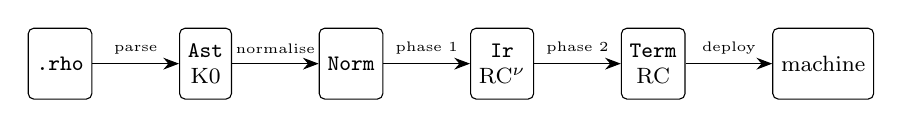
\begin{tikzpicture}[
  node distance=11mm,
  box/.style={draw, rounded corners=2pt, align=center, font=\footnotesize,
              minimum height=9mm, inner xsep=3pt},
  arr/.style={-{Stealth[length=2mm]}}]
\node[box] (txt) {\code{.rho}};
\node[box, right=of txt] (ast) {\code{Ast}\\K0};
\node[box, right=of ast] (norm) {\code{Norm}};
\node[box, right=of norm] (ir) {\code{Ir}\\$\mathrm{RC}^{\nu}$};
\node[box, right=of ir] (term) {\code{Term}\\$\mathrm{RC}$};
\node[box, right=of term] (mach) {machine};
\draw[arr] (txt) -- node[above, font=\tiny] {parse} (ast);
\draw[arr] (ast) -- node[above, font=\tiny] {normalise} (norm);
\draw[arr] (norm) -- node[above, font=\tiny] {phase 1} (ir);
\draw[arr] (ir) -- node[above, font=\tiny] {phase 2} (term);
\draw[arr] (term) -- node[above, font=\tiny] {deploy} (mach);
\end{tikzpicture}
\end{center}

\Fx{} gains \code{comb}, \code{comb-ir}, \code{comb-hash}, \code{comb-run} and
\code{comb-lattice}. \code{comb-run} \MUST{} reproduce the core-count
invariance \code{run} already has.

%======================================================================
\section{The lowering}\label{sec:lower}

\subsection{Phases}

\begin{enumerate}[leftmargin=1.6em]
\item Level check on the tree; guard check on the tree
(Requirement~\ref{req:guarded}); normalise; closedness check.
\item Phase one, per Definition~\ref{def:phase1}, producing IR.
\item Compute $\mathcal{F}(P)$ (Requirement~\ref{req:family}) and the leaf
demand (Requirement~\ref{req:fanout}).
\item Phase two, per unit (Requirement~\ref{req:units}), producing a closed
target term.
\item Encode, hash, and emit the artefact header: presentation, feature set,
erection construction, $\mathcal{F}(P)$, and the shapes available for a root
address.
\end{enumerate}

\begin{requirement}[Total and terminating, no Rust recursion]\label{req:total}
Both phases \MUST{} be total on terms passing the checks, \MUST{} terminate,
and \MUSTNOT{} recurse on the Rust stack, following the workspace rule.
\end{requirement}

\subsection{Occurrence analysis}\label{sec:occ}

\begin{table}[t]
\centering
\begin{tabularx}{\linewidth}{@{}llX l@{}}
\toprule
 & occurrence of $y$ & in the quoted body & link\\
\midrule
(o1) & input subject $\inp{z}{y}{S}$ & subject $\to c_{i}$ & $\bl(p_{i},c_{i})$\\
(o2) & output subject $\out{y}{S}$ & subject $\to c_{i}$ & $\br(p_{i},c_{i})$\\
(o3) & forwarded name $\out{v}{\drp{y}}$ & atom deleted & $\fw(p_{i},\enc{v})$\\
(o4) & drop $\drp{y}$ in process position & $\to \ev(c_{i})$ & $\fw(p_{i},c_{i})$\\
(o5) & inside a quotation $\quo{S}$, $y$ free in $S$ & subject $\to c_{i}$
     & constructor chain for $S$\\
\bottomrule
\end{tabularx}
\caption{The five occurrence kinds, \cite[Table~1]{draft3}.}
\label{tab:links}
\end{table}

\begin{requirement}[Classification]\label{req:classify}
For a receive with body $B$, the analysis \MUST{} collect every
\code{Name::Bound(d)} whose index equals the number of binders between it and
the receive, and assign each exactly one kind by this disjoint test on its
immediate role: the \code{chan} of a \code{Receive} bind, not under an
intervening quotation, is \textbf{o1}; the \code{chan} of a \code{Send},
likewise, is \textbf{o2}; the name of an \code{Eval} that is the sole argument
of a \code{Send} whose channel is not the occurrence is \textbf{o3}; the name
of an \code{Eval} in process position is \textbf{o4}; anything under an
intervening \code{Name::Quote} is \textbf{o5}, with the chain built for the
outermost such quotation. The tests \MUST{} be applied in that order. An
occurrence matching none \MUST{} raise an internal error naming the node.
\end{requirement}

\begin{requirement}[Coincident kinds]\label{req:coincide}
\cite[Table~1]{draft3}'s note about several kinds coinciding in one atom is
about occurrences, not kinds: each occurrence has one kind. The
implementation \MUST{} treat coincident occurrences independently, each with
its own bound name and link, in the order of
Requirement~\ref{req:occorder}, and \MUSTNOT{} fuse two occurrences into one
proxy. $R = \inp{y}{a}{\out{y}{\drp{y}}}$ of \S\ref{sec:thebug} is exactly
this case, and is the term on which the old scheme failed; fusing would
reintroduce a shared name within a single instance, which no amount of
per-instance allocation repairs.
\end{requirement}

\subsection{Constructor chains for (o5)}

\begin{requirement}[Chain construction]\label{req:chain}
For an (o5) occurrence inside the outermost enclosing quotation $\quo{S}$, the
compiler \MUST{} emit the chain rebuilding $\quo{\enc{S}}$ from the received
name and delivering it at $c_{i}$, by recursion on the path from the
occurrence to the root of $S$, per \cite[Prop.~3.12]{draft3}: the occurrence
itself needs no constructor; a parallel composition needs $\cons_{\mid}$; an
output needs $\cons_{\mm}$; an input needs $\cons_{\dd}$ when its bound name
occurs in its body and $\cons_{\sy}$ when it does not; every node off the path
is static and supplied as a constant message. Chains \MUST{} be built
outermost-last.
\end{requirement}

\begin{remark}[Proposition~3.12 is conditional, and its condition holds
here]\label{rem:prop311}
\cite[Prop.~3.12]{draft3} is stated for static apparatus, and
\cite[Rem.~3.13]{draft3} withdraws it for phase two. The distinction matters
for the implementation: the four constructors suffice for the \emph{(o5)
chains}, which rebuild source structure and whose shapes are those of the
source, while the \emph{erection} of phase two needs
$\mathcal{F}(P)$. These are two different demands on the family and
Requirement~\ref{req:family} takes their union.
\end{remark}

\begin{requirement}[No repeated subject in a constructor]\label{req:norepeat}
A constructor \MUSTNOT{} be emitted with two equal argument channels, nor with
a delivery channel among its inputs (\cite[Rem.~3.4]{draft3}). Where the same
value is needed twice, the compiler \MUST{} split with $\dd$ first. A join
group with a repeated channel is not a request for two data at that channel.
\end{requirement}

\subsection{Shortcuts}

\begin{requirement}[Feature-gated, and they enlarge the family]
\label{req:shortcuts}
\cite[Rem.~6.4]{draft3} gives three cheaper cases and states, following
\cite[Rem.~3.13]{draft3}, that they are not free: they put a bound name into
the argument of an $\ev$ or a $\fw$, so they add $\cons_{\ev}$ and
$\cons_{\fw}$ to $\mathcal{F}(P)$. Under
\cite[Lem.~6.14]{draft3} this no longer threatens freshness, which is by size
rather than by shape, but it does change $\mathcal{F}(P)$, the lattice point
and every content hash. The feature \MUST{} be off by default and recorded in
the artefact header.
\end{requirement}

\subsection{Worked examples}

\begin{requirement}[Three golden traces]\label{req:golden}
The following \MUST{} be golden files --- source, IR, target, encoding, hash,
and the full reduction sequence with step counts:
\begin{enumerate}[leftmargin=1.8em,label=(\roman*)]
\item $W$ of \S\ref{sec:thebug}, the term the two phases exist for, asserting
the observation at $\enc{\quo{X}}$ and, explicitly, the \emph{absence} of the
crossed residue (Requirement~\ref{req:Wtest});
\item $\enc{W}$ at phase one, asserting that the two instances of $R$ are
$\alpha$-distinct (\cite[Ex.~6.5]{draft3});
\item $D_{x} = \inp{y}{x}{(\out{x}{\drp{y}} \mid \drp{y})}$, the recursion
combinator, whose run \cite[Ex.~6.9]{draft3} works out in full: seven bound
names, the erection, the eight reduction steps, and the residue at a strictly
deeper address.
\end{enumerate}
Goldens \MUST{} be regenerated only by an explicit command.
\end{requirement}

\begin{requirement}[Output size]\label{req:size}
$|\enc{P}^{\sharp}| = O(|P|)$ under either conforming scheme of
Section~\ref{sec:schemes}: the curried scheme emits one constructor and one
$\dd$ per erected atom with the paths as parameters, and $\inst$ emits two
atoms per unit. The logarithmic factor \cite[Prop.~8.1]{draft3} folds in is a
\emph{name}-size figure, $|\sigma\!\cdot\!w| = |\sigma| + O(|w|)$, and \MUST{}
be reported as one rather than as an atom count. On the nesting family of
\cite[Prop.~8.2]{draft3} phase one \MUST{} give $3d+1$ atoms against Yoshida's
$(3^{d-1}+1)/2$, tested as a law parameterised over $d$; phase two multiplies
by a constant, which \MUST{} be measured and reported rather than asserted.
\end{requirement}

%======================================================================
\section{The machine}\label{sec:runtime}

\subsection{The instantiation}

Every rule of Definition~\ref{def:tred} consumes messages at one to $n$ named
subjects and produces messages or atoms. There is no pattern to match beyond
the subject, no binder to open, no substitution. \Camp{} is exactly that
store, with joins for the multi-subject case.

\begin{decision}[The machine is \Camp{} with a three-line matcher]
\label{dec:machine}
\code{f1r3comb-run} \MUST{} be \code{campf1r3-core::Space} instantiated over
target terms and \MUSTNOT{} implement its own indexing, joins or replay. The
spatial matcher of \code{k1ndl1ng-campf1r3} is not used and \MUST{} not be
linked.
\end{decision}

\begin{center}
\begin{tabularx}{\linewidth}{@{}l>{\raggedright\arraybackslash}X@{}}
\toprule
\Camp{} parameter & \Comb{} instance\\
\midrule
$C$, channel & \code{CName}, a target name, hashed by its encoding\\
$A$, datum & \code{enum Val \{ Loud(CName), Quiet(Term) \}} --- the sorts of
$\mm$ and $\qq$ differ under A, so an enum over two types, not a struct with a
flag\\
$P$, pattern & \code{Acc \{ accepts\_quiet: bool \}}\\
$K$, continuation & \code{Rule}, from the generated shape table\\
$M$, matcher & reject a quiet datum for a non-forwarder pattern; otherwise
accept\\
$O$, observer & \code{NoObserver} at v1\\
\bottomrule
\end{tabularx}
\end{center}

\begin{requirement}[Joins are variable-arity]\label{req:joins}
With $\cons_{A}$ a schema, a constructor's join group has $\mathrm{ar}(A)$
channels. The deploy path \MUST{} issue
\code{consume(channels, patterns, k)} with the group read off the generated
table, and \MUSTNOT{} assume two or three. \Camp{} supports joins of arbitrary
group size; the implementation \MUST{} nonetheless bound the arity and
diagnose a shape whose arity exceeds it.
\end{requirement}

\begin{requirement}[$\mathsf{eval}$ normalises before it deploys]
\label{req:evalnorm}
Under A the rule produces $\drp{v}$, whose normal form is the process $v$
quotes. The machine \MUST{} construct $\drp{v}$ through the smart constructor,
which performs the elimination, and deploy the result. It \MUSTNOT{}
short-circuit by projecting the payload out of the name: the short-circuit is
observationally identical here and is the step that becomes unsound under
\code{presentation-b}.
\end{requirement}

\begin{requirement}[Linear, never persistent]\label{req:linear}
Every \code{consume} \MUST{} pass \code{persist = false} and an empty
\code{PeekSet}; \code{install} \MUSTNOT{} be used. Every rule consumes its
participants, and there is no persistent atom in the calculus.
\end{requirement}

\subsection{Addresses}

\begin{requirement}[The address allocator]\label{req:allocator}
The machine \MUST{} own an address allocator satisfying
Requirements~\ref{req:rootaddr} and~\ref{req:addrsep}: it hands each deploy a
root address of a shape outside that program's family, prefix-incomparable
with every address in use, and posts it at the unit's $r$. It \MUST{} record
addresses in the event stream, because an address is the only thing that
distinguishes two instances and a trace without them is unreadable.
\end{requirement}

\begin{hazard}[Addresses grow without bound]\label{haz:growth}
Every self-instantiation descends one level: \cite[Ex.~6.9]{draft3}'s residue
sits at a strictly deeper address, and $|\Lft\sigma| = |\sigma| + O(1)$. A
recursive program therefore grows its channel keys linearly in the number of
unfoldings, and a program that builds names from constructed names doubles
them. \cite[\S12]{draft3} open question~3 and \cite[\S7]{logic} both name
this; under phase two it is no longer a pathological case but the normal
behaviour of every loop.
\end{hazard}

\begin{requirement}[Interning and budget]\label{req:intern}
Constructed names \MUST{} be hash-consed, with the encoding stored once and
channels referring to it by index, and the representation \SHOULD{} share the
common prefix of an address spine so that descending one level costs $O(1)$
rather than $O(|\sigma|)$. The machine \MUST{} accept a budget --- maximum
name size, maximum distinct names --- and halt with
\code{comb-name-budget} naming the constructor or the unfolding that exceeded
it. Because Hazard~\ref{haz:growth} now fires on ordinary recursive programs,
the budget \MUST{} be a supported operational parameter and not a debugging
aid, and the measured growth rate \MUST{} be reported by
\code{comb-run --trace}.
\end{requirement}

\begin{requirement}[Races are scheduler choices and \MUST{} be visible]
\label{req:races}
\cite[\S3.3]{draft3} records two deliberate races, and phase two adds a third:
every cross-match at a static channel between concurrent instances
(\cite[Rem.~6.10]{draft3}). The machine \MUST{} emit a trace event at each
resolution naming the alternatives not taken and the addresses involved. This
is not only for \Rhobots: it is the instrumentation
Obligation~\ref{obl:permutetest} needs, since a counterexample to permutation
invariance will appear first as a cross-match followed by a divergence.
\end{requirement}

%======================================================================
\section{The lattice audit}\label{sec:lattice}

\begin{requirement}[Report both phases]\label{req:lattice}
\code{f1r3comb-lower} \MUST{} return the atom multiset of \emph{both} images,
and \code{f1r3x comb-lattice} \MUST{} print both points. \cite{logic} revision~2 now says the same
from the logic's side: phase-two images all sit near the top of both axes,
while occupancy is informative for phase-one images. Under
\code{inst-erection} the phase-two point degenerates completely to a single
shape (Requirement~\ref{req:instfeature}), which is one of the three reasons
behind Decision~\ref{dec:scheme}. Reporting only the target would make the
audit look like a constant function and would waste
\cite[Thm.~6.5]{logic}.
\end{requirement}

\begin{requirement}[Model checking a compiled program is not decidable]
\label{req:mcundec}
\cite{logic} revision~2 records a consequence the compiler should surface
rather than let a user discover: the decidability of its
Proposition~\ref{sec:lattice}-adjacent modal fragment assumes
$\ev \notin \Atm$, and every compiled unit with an input contains $\ev$ ---
in the gate \cite[Lem.~6.2]{draft3}, and once per erected atom
\cite[Rem.~3.11]{draft3}. \code{comb-lattice} \MUST{} therefore report, for
each image, whether it falls in the decidable fragment, and \MUST{} say
plainly that a phase-two image of a program with an input does not.
\end{requirement}

\begin{requirement}[The multiset is the logic's input]\label{req:logicinput}
\code{f1r3comb-term} \MUST{} expose the atom multiset and the encoding through
a stable API so the occupancy checker of \cite[\S6]{logic} can be built
against it, preserving the $\mm$/$\qq$ sort distinction on which
\cite[Rem.~2.5]{logic} turns. It \SHOULDNOT{} expose more.
\end{requirement}

\begin{requirement}[The weighted count]\label{req:weighted}
Where the implementation computes the halting bound of
\cite[Prop.~9.9]{draft3} --- in the budget of Requirement~\ref{req:intern}, in
the lattice report, or in a test --- it \MUST{} use the \emph{weighted} count
of \cite[Def.~6.6]{logic}, in which $\bl$, $\br$ and $\sy$ count twice,
because those rules consume themselves and produce an $\fw$ and so preserve
rather than decrease the plain count. The unweighted count bounds the weighted
one only by a factor of two.
\end{requirement}

%======================================================================
\section{Correctness obligations and testing}\label{sec:test}

\begin{obligation}[The $W$ regression]\label{obl:W}
Requirement~\ref{req:Wtest}. $W$ run under the machine \MUST{} produce the
observation the source produces, and \MUST{} not produce the crossed residue.
A variant with three messages at $a$ and a body of three drops \MUST{} also be
tested, since two instances can be crossed by accident and three cannot.
\end{obligation}

\begin{obligation}[Discipline conformance, and permutation tested anyway]
\label{obl:permutetest}
\cite[Lem.~6.11]{draft3} proves permutation invariance for images satisfying
\cite[Def.~6.10]{draft3}, so the primary evidence is now the conformance check
of Requirement~\ref{req:sai}, which \MUST{} be a unit test on every corpus
term and not only a compile-time assertion. The behavioural test remains
worth running, because conformance is a property of the emitted term and the
machine could still break the lemma's hypothesis --- by handing out comparable
addresses, or by consuming a leaf twice. So: for a corpus of terms with $k \geq 2$ concurrent
instances of one unit, run under a scheduler that \emph{maximises}
cross-matching at static channels --- an adversarial profile that, at each
choice point, prefers the datum from the instance that did not produce it ---
and compare observations against \Bell. The deterministic profile will rarely
exhibit the interleaving; a test that only runs deterministically tests
nothing here. The adversarial profile \MUST{} be a supported \Camp{} strategy
in \code{f1r3comb-check}. A term that fails this while passing
Requirement~\ref{req:sai} is a counterexample to
\cite[Lem.~6.11]{draft3} and \MUST{} be reported as such rather than patched.
\end{obligation}

\begin{obligation}[The mixing experiment, reproduced]\label{obl:mixing}
\code{phase2-results.txt} is a reproducible result and \MUST{} be reproduced
by \code{f1r3comb-check}: the literal erection of
\cite[Def.~6.8]{draft3} mixes in 29 of 50 runs at two instances and 50 of 50
at eight or more, under the parallel schedule, and the conforming scheme mixes
in none at any instance count under either schedule. The test \MUST{} run the
non-conforming construction deliberately, as a negative control, since a suite
that can only build conforming terms cannot demonstrate that conformance is
what is doing the work. The $D_{x}$ figures --- seven parallel steps and
sixteen new names per unfolding, constant over two hundred unfoldings and
independent of address depth --- \MUST{} be asserted as a regression on
Requirement~\ref{req:intern}'s prefix sharing.
\end{obligation}

\begin{obligation}[The marking analysis]\label{obl:marking}
Requirement~\ref{req:marking}. For a corpus, the marking \MUST{} agree with a
brute-force check: a unit is safe for the fixed-arity family exactly when no
crossing of instances changes the observation, determined by exhaustive
scheduling at two and three instances. $\inp{y}{a}{(\drp{y} \mid \drp{y})}$
\MUST{} come out safe and $R$ \MUST{} come out unsafe
(Requirement~\ref{req:deciding}); a marking that cannot tell them apart is
not the analysis \cite[Rem.~6.20]{draft3} describes.
\end{obligation}

\begin{obligation}[Canonicity]\label{obl:canon}
For randomly generated K0 terms and $\scong$-variants obtained by permuting
parallel components and re-associating, the compiled encodings \MUST{} be
byte-equal, at both phases.
\end{obligation}

\begin{obligation}[The conflation regression]\label{obl:defect}
A test \MUST{} assert that $Q \mid \mm(\quo{Q},\quo{P})$ is stuck for a
nontrivial $Q$ --- that the machine does not implement
\cite[Prop.~3.5]{draft3} --- and a second \MUST{} assert rigidity: no process
is equal to an $\ev$ atom unless written as one.
\end{obligation}

\begin{obligation}[Freshness]\label{obl:fresh}
Three checks, all cheap under \cite[Lem.~6.14]{draft3}. The root address
exceeds the largest name of $\enc{P}$ (Requirement~\ref{req:rootaddr}); the
static channels do too (Requirement~\ref{req:staticfresh}); and no
address-derived channel supplies a value to an (o5) chain
(Requirement~\ref{req:o5noaddr}). A property test \MUST{} include the
adversarial source term $\quo{(\out{x}{\nil})}$, whose encoding is
$\Lft\enc{\quo{x}}$ --- a leaf of the address $\enc{\quo{x}}$ --- since it
passes any test that checks only distinctness of leaves from one another, and
is excluded here only by the size condition.
\end{obligation}

\begin{obligation}[Operational correspondence]\label{obl:opcorr}
\cite[Lem.~7.7]{draft3} fixes the reduction sequence after a communication.
The machine \MUST{} be tested against the step counts for a corpus with known
$k$, now including the phase-two overhead: three steps per allocation gadget
(\cite[Lem.~6.7]{draft3}) and two per erected atom
(\cite[Rem.~3.11]{draft3}).
\end{obligation}

\begin{obligation}[Differential testing against \Bell]\label{obl:diff}
For a corpus of K0 programs, run the source under \Bell{} and the compiled
term under \code{f1r3comb-run} to quiescence and compare observations. The
observation \MUST{} be the multiset of messages at names that are encodings of
source names --- the encoded observer class of \cite[Thm.~7.9]{draft3} --- and
\MUSTNOT{} include allocated leaves or static channels, which by
\cite[Lem.~7.6]{draft3} no encoded context can name.
\end{obligation}

\begin{obligation}[A against B]\label{obl:AB}
The corpus \MUST{} be run under both presentations, unscoped: with
\cite[Def.~3.8]{draft3}'s member for shapes with a process argument, B
expresses the whole translation, and v0.3's exclusion is withdrawn
(Remark~\ref{rem:withdrawn}). The two readings of $\cons_{\qq}$ \MUST{}
additionally be compared atom by atom on every erected gate
(Requirement~\ref{req:consq}).
\end{obligation}

\begin{obligation}[Property tests]\label{obl:prop}
On generated K0 terms: both phases total; no binder in the target
(Requirement~\ref{req:novars}); no drop under A; no constructor with a
repeated or self-delivering channel; the family is one level deep
(Requirement~\ref{req:family}); leaf demand matches supply
(Requirement~\ref{req:fanout}); one spare per nested unit
(Requirement~\ref{req:spares}); size bounds
(Requirement~\ref{req:size}); deploy-then-quiesce terminates for terminating
sources.
\end{obligation}

\begin{obligation}[Address independence]\label{obl:addr}
\cite[Lem.~7.8]{draft3}: a unit run at $\sigma$ and at $\tau$
prefix-incomparable are bisimilar. Tested by running the corpus at two
unrelated root addresses and comparing observations. A failure here is a
machine bug, not a compiler bug.
\end{obligation}

%======================================================================
\section{Errors and diagnostics}\label{sec:errors}

\begin{center}
\begin{tabularx}{\linewidth}{@{}ll>{\raggedright\arraybackslash}X@{}}
\toprule
Code & Phase & Meaning\\
\midrule
\code{comb-level} & 1 & A form above K0\\
\code{comb-unguarded-drop} & 1 & A drop of a name not bound by an enclosing
input; warning under A, error under B\\
\code{comb-drop-quote} & 1 & A literal $\drp{\quo{Q}}$\\
\code{comb-open}, \code{comb-unforgeable} & 1 & Grounding survived, or an
unforgeable name\\
\code{comb-occ-unclassified} & 2 & Internal: an occurrence matching no kind\\
\code{comb-arity} & 4 & A shape whose constructor arity exceeds the join bound
(Requirement~\ref{req:joins})\\
\code{comb-discipline} & 4 & The emitted image violates
\cite[Def.~6.10]{draft3} (Requirement~\ref{req:sai})\\
\code{comb-scheme-mismatch} & deploy & Artefact header names a different
erection scheme (Decision~\ref{dec:scheme})\\
\code{comb-o5-address} & 4 & An address-derived channel feeds an (o5) chain
(Requirement~\ref{req:o5noaddr})\\
\code{comb-static-not-fresh} & deploy & A static channel does not exceed the
largest name of $\enc{P}$ (Requirement~\ref{req:staticfresh})\\
\code{comb-address-too-small} & deploy & The root address does not
(Requirement~\ref{req:rootaddr})\\
\code{comb-address-overlap} & deploy & A root address comparable with one in
use (Requirement~\ref{req:addrsep})\\
\code{comb-presentation-mismatch} & deploy & Artefact header disagrees\\
\code{comb-name-budget} & run & Name size or count exceeded\\
\code{comb-decode} & any & A source tag, or the drop tag under A, where a
target tag was expected\\
\bottomrule
\end{tabularx}
\end{center}

%======================================================================
\section{Performance and portability}\label{sec:perf}

\begin{requirement}[Complexity]\label{req:complexity}
Phase one \MUST{} be linear in the source normal form. Phase two \MUST{} be
linear in the phase-one image, or $O(n \log n)$ under
Section~\ref{sec:schemes}. Encoding \MUST{} be linear and computed once per
node. A machine step \MUST{} be $O(1)$ expected in the size of the store,
\emph{given} the prefix sharing of Requirement~\ref{req:intern}; without it,
hashing an address of depth $d$ is $O(d)$ and a recursive program degrades
quadratically, which \MUST{} be a measured test and not an assumption.
\end{requirement}

\begin{requirement}[Targets]\label{req:targets}
Compile a $10^{4}$-node source term in under 10\,ms; deploy $10^{5}$ atoms in
under 100\,ms; sustain $10^{6}$ machine steps per second free-running; and
sustain $10^{4}$ unfoldings of $D_{x}$ without the step cost rising, which is
the test that Requirement~\ref{req:intern}'s prefix sharing works. Budget
figures, to be re-stated once measured.
\end{requirement}

\begin{requirement}[Portability and determinism]\label{req:port}
Every crate \MUST{} build for \code{wasm32-unknown-unknown} without
\code{wasm-bindgen}, carry \code{forbid(unsafe\_code)}, and take no external
dependency. Given the same source, presentation, construction and root
address, the compiled term, its encoding, its hash, the event stream and the
final scene \MUST{} be bit-identical across runs, hosts, core counts and
WebAssembly versus native.
\end{requirement}

%======================================================================
\section{What the implementation asks of the papers}\label{sec:paper}

Three of v0.4's items are discharged, and the first is discharged by being
overtaken: \cite[\S6.6]{draft3} not only confirms that $\ERECT$ fails the
discipline but shows the obstruction is structural, which is a stronger and
more useful result than the one asked for. The two-stage construction v0.4
offered is refuted (Remark~\ref{rem:twostagegone}). The remaining items:

\begin{enumerate}[leftmargin=1.8em]

\item \textbf{The comparison table over-counts against the curried scheme}
(Remark~\ref{rem:tablerow}). \cite[\S6.7]{draft3} marks the allocation tree
and gadget channels as still needed for curried and removed for $\inst$. Since
$\cons^{*}_{A}[\vec w]$ derives $\sigma\!\cdot\!w_{i}$ inside its own rule, no
leaf needs a channel, the $\ALLOC$ gadget of Definition~6.6 goes, and with it
the per-node channels of Remark~6.13 and the fan-out bookkeeping. What remains
is one $\dd$ per erected atom. Proposed amendment: correct the row, which
narrows the gap the recommendation rests on.

\item \textbf{The measurements have no curried arm}
(Remark~\ref{rem:thirdarm}). \code{phase2-results.txt} compares literal
against context. The literal result is decisive and settles that the
construction is broken. Nothing in the file bears on $\inst$ versus curried,
and \cite[Rem.~6.22]{draft3} says so; a third arm in \code{phase2.py} is cheap
and would settle it.

\item \textbf{$\inst$'s cost is not only conceptual}
(Remark~\ref{rem:whycurried}). \cite[Rem.~6.22]{draft3} calls the price ``an
atom parameterised by a context''. Two further consequences are worth
recording where the recommendation is made: the two-step figure hides
$O(|{\rm unit}|)$ work in one rule application, so a cost-accounted variant
must charge $\inst$ by size and not by step; and $C[v]$ is substitution under
quotation, which \cite[\S3.6]{draft3} identifies as the operation the
constructor family exists to simulate, so taking it as primitive gives up the
property that a rule's right-hand side is built from names by fixed shape
formers. On a machine that property is what makes the runtime a store with a
three-line matcher.

\item \textbf{$\inst$ has no home in \cite{logic}.} Revision~2 restates
$\Atm_{\mathrm{full}}$ as the base atoms, $\cons_{\mid}$, and one constructor
per shape a program erects, every production being a schema over shapes. The
curried family is that shape set with a path tuple as a parameter; $\inst$'s
third argument is a term with holes, so it has no structural production, no
occupancy disjunct and no position on either axis. Proposed amendment: say
which of the two schemes \cite{logic} is to be read over, since the two notes
currently point in different directions.

\item \textbf{No freshness condition on the static channels}
(Erratum~\ref{err:staticfresh}). From v0.4 and still open.
\cite[Lem.~6.14]{draft3} makes the leaves fresh against $\nms{\enc{P}}$;
nothing makes $r$ or the $f_{A}$ fresh, and an encoded context that names $r$
posts an address of its choosing, defeating the hypotheses of both
\cite[Lem.~6.11]{draft3} and \cite[Lem.~6.14]{draft3}. The same size argument
fixes it.

\item \textbf{The enumeration order of occurrences is observable}
(Requirement~\ref{req:occorder}), and \textbf{coincident occurrence kinds}
(Requirement~\ref{req:coincide}). From v0.2, still open, and the second is now
pointed at by the paper's own examples: $R$ is the coinciding case, and
\cite[Ex.~6.21]{draft3} is what it costs to get it wrong.

\item \textbf{The formation table's $\mm$ row is presentation-specific},
seconded from \cite[Rem.~2.6]{logic}; and \textbf{\cite[\S2]{draft3}'s source
calculus is not \cite[Def.~2.6]{k1ndl1ng}'s}
(Obligation~\ref{obl:srcagree}), the two agreeing exactly on guarded-drop
terms.

\end{enumerate}

%======================================================================
\section{Open questions}

\begin{enumerate}[leftmargin=1.8em]
\item \textbf{Address growth, measured} (Hazard~\ref{haz:growth}). Under phase
two every loop descends, so this is now the common case rather than the
pathological one. Does a real program need address compaction --- reusing a
retired subtree --- and is that safe?
\item \textbf{Is the full family necessary?} \cite[\S12]{draft3} asks it and
\cite[Rem.~6.15]{draft3} narrows it to the shapes a program erects. With
freshness now by size rather than by shape, the question is no longer
load-bearing for correctness, only for the atom count and the lattice point.
\item \textbf{Receptivity} (\cite[open item~5]{logic}). If the logic gains it,
the $\mm$/$\qq$ argument for A weakens, and with
Remark~\ref{rem:withdrawn} the balance on storage already leans the other way;
what would not move is the injectivity of quotation.
\item \textbf{An optimising decoder.} The one development that would force B,
and no longer blocked by anything in phase two (Remark~\ref{rem:withdrawn}).
\item \textbf{The matrix encoding.} A reduction graph as an upper-triangular
matrix wants a bounded name universe; phase two makes the universe grow with
every unfolding, which is a real constraint on that programme and worth
stating before it is designed around.
\item \textbf{Composition with the $\pi$ compiler}, and \textbf{a decompiler}
as a round-trip canonicity check.
\end{enumerate}

%======================================================================
\section{Delivery}

\begin{center}
\begin{tabularx}{\linewidth}{@{}ll>{\raggedright\arraybackslash}X@{}}
\toprule
M & Deliverable & Done when\\
\midrule
M0 & \code{f1r3comb-term} & Shape table, generated atoms and constructors,
drop elimination, encoding, hash, decoder, multiset; tag and rigidity tests\\
M1 & \code{f1r3comb-ir}, phase one & Binder, de Bruijn, extrusion,
$\alpha$-equivalence; checks; occurrence analysis; (o5) chains; canonicity
property test; golden (ii)\\
M2 & Phase two & Family computation, the marking analysis
(Requirement~\ref{req:marking}), the erection scheme of
Decision~\ref{dec:scheme}, spares, fan-out; the
\cite[Def.~6.10]{draft3} conformance pass and the (o5) address pass; golden
(iii), the $D_{x}$ run\\
M3 & \code{f1r3comb-space}, \code{f1r3comb-run} & Matcher, generated rule
table, address allocator, deploy, trace; conflation and freshness regressions\\
M4 & \code{f1r3comb-check} & Golden (i), the $W$ regression; the adversarial
scheduler and Obligation~\ref{obl:permutetest}; differential testing\\
M5 & \Fx{}, WASM & The five subcommands; \code{wasm32}; performance measured
and Requirement~\ref{req:targets} re-stated\\
\bottomrule
\end{tabularx}
\end{center}

\noindent
The weight has shifted again, and in the right direction. Under v0.3 the
differential test was the only evidence for phase two's central invariant;
with \cite[Lem.~6.11]{draft3} proved, the primary evidence is the conformance
check of Requirement~\ref{req:sai}, which belongs to M2 and costs a dataflow
pass. M4 returns to being a confidence measure --- with the adversarial
scheduler retained, because the lemma's hypotheses are about the machine as
much as the term.

%======================================================================
\section{Changes from v0.4}\label{sec:v4delta}

\begin{center}
\begin{tabularx}{\linewidth}{@{}l>{\raggedright\arraybackslash}X@{}}
\toprule
v0.4 & v0.5\\
\midrule
Requirement 5.15, $\ERECT$ does not conform & Confirmed and strengthened by
\cite[\S6.6]{draft3}; kept as Requirement~\ref{req:erectviolates}, now with
\cite[Ex.~6.16]{draft3} behind it\\
Requirement 5.16, two-stage erection & \textbf{Withdrawn.} The regress of
\cite[\S6.6]{draft3} eats stage~(ii), and
\cite[Prop.~6.17]{draft3} shows no fixed-arity construction reaches the atoms
at all (Remark~\ref{rem:twostagegone})\\
--- & New: Decision~\ref{dec:scheme}, the erection scheme, curried by default
with $\inst$ behind a feature, and Remarks~\ref{rem:thirdarm}
to~\ref{rem:whycurried} for the argument\\
--- & New: Requirement~\ref{req:marking}, the decidable marking analysis of
\cite[Rem.~6.20]{draft3}, which lets a unit with no atom mentioning two marked
names keep the cheap construction\\
--- & New: Requirement~\ref{req:deciding} and
Obligation~\ref{obl:mixing}, the deciding term, its near miss, and the
reproduction of \code{phase2-results.txt} with the broken construction kept as
a negative control\\
Requirements 5.9, 5.11, 5.12, allocation gadget, spares, fan-out & Retained
but scheme-dependent: the $\ALLOC$ gadget disappears under both conforming
schemes, spares become paths, fan-out is of the address\\
Lattice report informative at phase one & Plus
Requirement~\ref{req:mcundec}: every compiled unit with an input contains
$\ev$, so no such image falls in the logic's decidable modal fragment ---
\cite{logic} revision~2's own note, surfaced by the tool\\
$|\enc{P}^{\sharp}| = O(|P|\log|P|)$ & $O(|P|)$ atoms; the logarithm is a
name-size figure and \MUST{} be reported as one\\
Six items asked of the papers & Seven, of which three are discharged and four
are new\\
\bottomrule
\end{tabularx}
\end{center}

%======================================================================
\begin{thebibliography}{99}

\bibitem{bytecode} F1R3FLY.io.
\emph{Bytecode or normal form: what the executive should execute.}
\code{publications/campf1r3/bytecode-or-normal-form}, 2026.

\bibitem{campf1r3} F1R3FLY.io.
\emph{CampF1R3: an in-memory tuple space.}
\code{publications/campf1r3/campf1r3-spec}, 2026.

\bibitem{draft3} L.\,G. Meredith and M. Stay.
\emph{Name-free combinators for the rho calculus: a repair, a linear encoding,
and the one operation that was missing.} Draft~3,
\code{publications/rho-combinators}, September 2026.

\bibitem{logic} F1R3FLY.io.
\emph{A spatial-behavioural logic for the rho combinators.} Draft~2,
revision~1, \code{publications/rho-combinators}, 22 September 2026.

\bibitem{k1ndl1ng} F1R3FLY.io.
\emph{K1ndl1ng: a parser and a normaliser for the kernel of rholang.}
Specification v0.2, \code{publications/campf1r3/k1ndl1ng-spec}, 2026.

\bibitem{MeredithRadestock05} L.\,G. Meredith and M. Radestock.
\emph{A reflective higher-order calculus.} ENTCS 141(5):49--67, 2005.

\bibitem{nowns} L.\,G. Meredith.
\emph{Namespaces without a name server.} \code{publications/pi2rhobugfix},
F1R3FLY.io, 2026.

\bibitem{rhocomb} L.\,G. Meredith and M. Stay.
\emph{Name-free combinators for concurrency.} Working draft, \code{rho4u}.

\bibitem{Yoshida02} N. Yoshida.
\emph{Minimality and separation results on asynchronous mobile processes.}
Theoretical Computer Science 274(1--2):231--276, 2002.

\end{thebibliography}

\end{document}
